% Chapter 3: Methodology

This chapter describes the methods and approaches used in the experiments. This includes dataset preparation, models, loss functions, etc.

\section{Overview of Approach}
An overall description of the approach to tackling the long-tailed dataset problem, including an explanation of the strategy, 
such as balancing techniques and model selection.

\section{Dataset Preparation and Specifications}
A description of this section here.

Following the dataset structure used in \textit{Deep Long-Tailed Learning: A Survey}, the CIFAR100 dataset was modified to create a long-tailed training set and a balanced test set. Key details include:

\begin{itemize}
    \item Dataset characteristics: Number of classes, imbalance ratio, and train-test splits.
    \item Preprocessing steps: Resizing, normalization, and augmentation techniques.
    \item Handling imbalance: Techniques like re-sampling and augmentation to address the long-tailed distribution.
\end{itemize}

\subsection{Data Characteristics: Class Distribution}
\textit{A list of subjects to include in this section:}

\begin{itemize}
    \item Describe the ImageNet-LT dataset: number of classes, imbalance ratio, etc.
    \item Describe the plots and what they mean for the CIFAR100-LT data preparation. 
\end{itemize}

The first step is to prepare the data for training and testing. In order to generate training, validation, and test datasets that resemble the datasets used for the empirical studies in \textit{Deep Long-Tailed Learning: A Survey} \cite{zhang2023deep}, their dataset are investigated: The GitHub repository \cite{VanintLT} for the paper \textit{Deep Long-Tailed Learning: A Survey} was downloaded and an environment was set up on the Jupyter Hub on the Freja node on the ece cluster. The \texttt{.txt} files with the data from ImageNet-LT (\texttt{ImageNet\_LT\_train.txt}, \texttt{ImageNet\_LT\_val.txt}, \texttt{ImageNet\_LT\_test.txt}) are shown on figures \ref{fig:IN-train}, \ref{fig:IN-val}, and \ref{fig:IN-test}, respectively. 

\begin{figure}[h!]
    \centering
    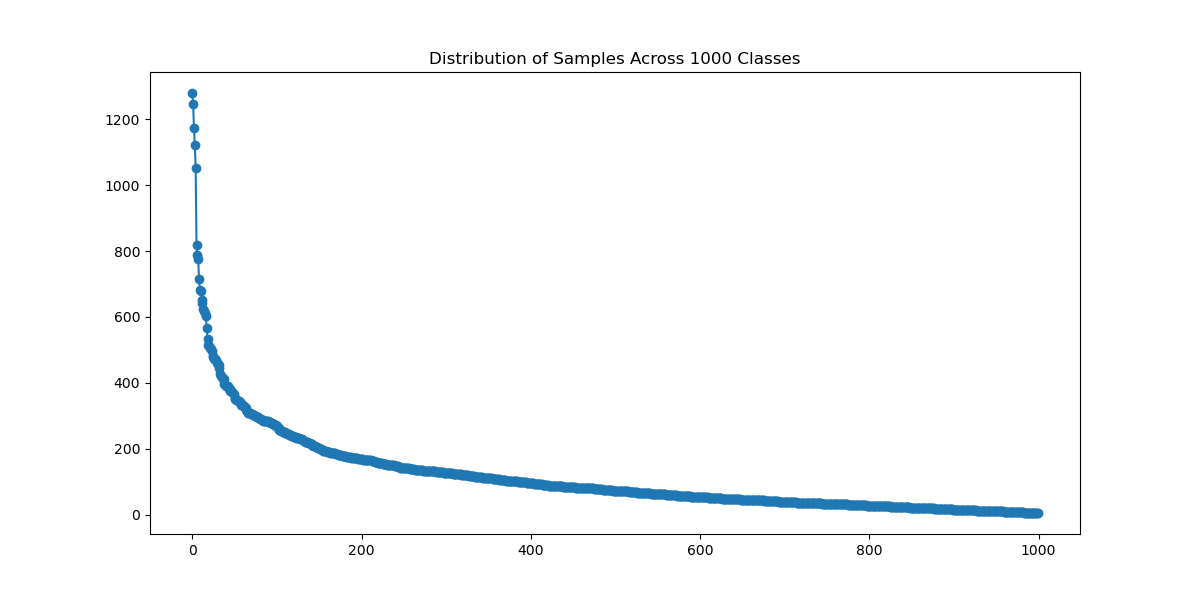
\includegraphics[width=0.9\textwidth]{Images/Plots/class_distribution_train.png}
    \caption{The class distribution of the training images for the ImageNet-LT dataset shows a long-tailed distribution.}
    \label{fig:IN-train}
\end{figure}

\begin{figure}[H]
    \centering
    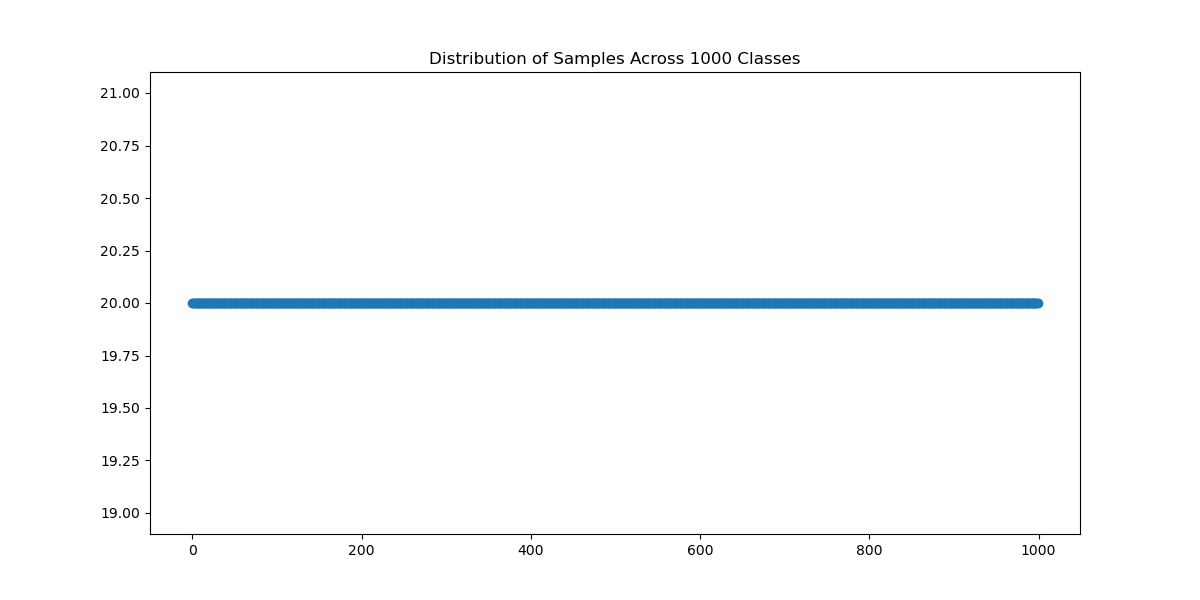
\includegraphics[width=0.9\textwidth]{Images/Plots/class_distribution_val.png}
    \caption{The class distribution of the validation images for the ImageNet-LT dataset shows that there are 20 samples of each class.}
    \label{fig:IN-val}
\end{figure}

\begin{figure}[H]
    \centering
    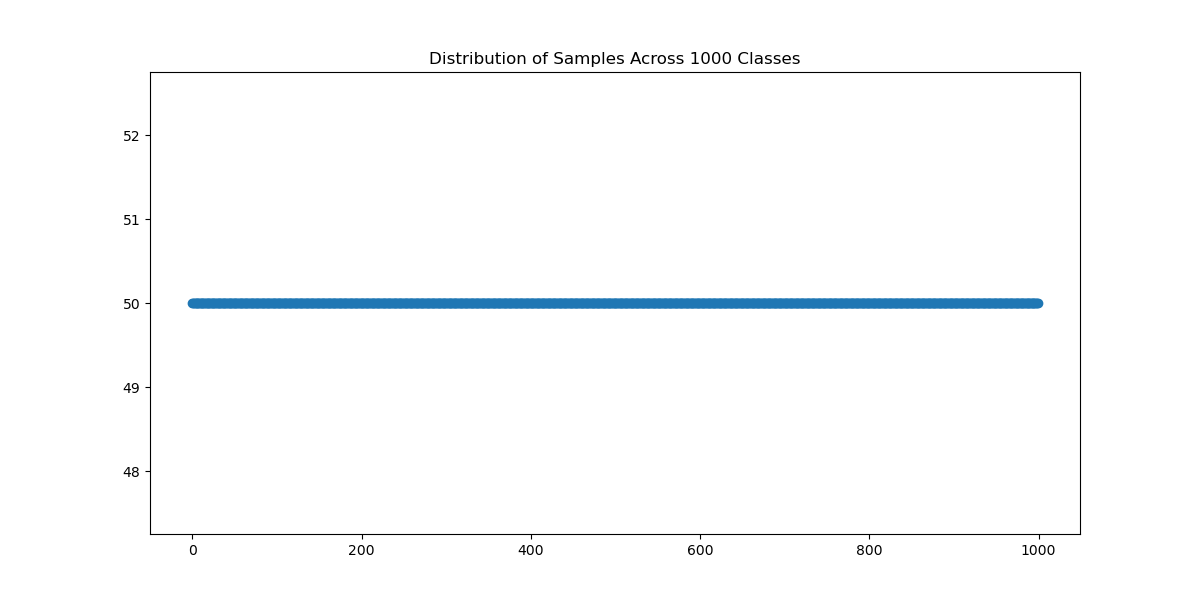
\includegraphics[width=0.9\textwidth]{Images/Plots/class_distribution_test.png}
    \caption{The class distribution of the test images for the ImageNet-LT dataset shows that there are 50 samples of each class.}
    \label{fig:IN-test}
\end{figure}

\subsection{Preparation: CIFAR100-LT}
\textit{A list of subjects to include in this section:}

\begin{itemize}
    \item Briefly describe the CIFAR100 dataset, and why it was chosen as the primary dataset for this thesis. Refer to section 2.1.
    \item Insert plots of the CIFAR100 dataset.
    \item Describe the generation of the imbalanced dataset: IMBALANCECIFAR100 method from the LDAM-DRW paper.
    \item Describe the imbalance ratio.
    \item Explain why the dataset was saved, and not generated in run-time, like in LDAM-DRW.
    \item Explain why the dataset was split into 450 samlpes per class for training and 50 samples per class for testing.
    \item Insert plots of the imbalanced dataset.
    \item Describe the head, middle, and tail classes.
    \item Insert plot of the division of the long-tailed test dataset: head, middle, and tail classes.
    \item Explain the purpose of the division.
    \item Potentially a few images from the CIFAR100 dataset.
\end{itemize}

Describe the class distribution in figures \ref{fig:cifar100_imbalance_cifar} and \ref{fig:cifar100val}.

\begin{figure}[H]
    \centering
    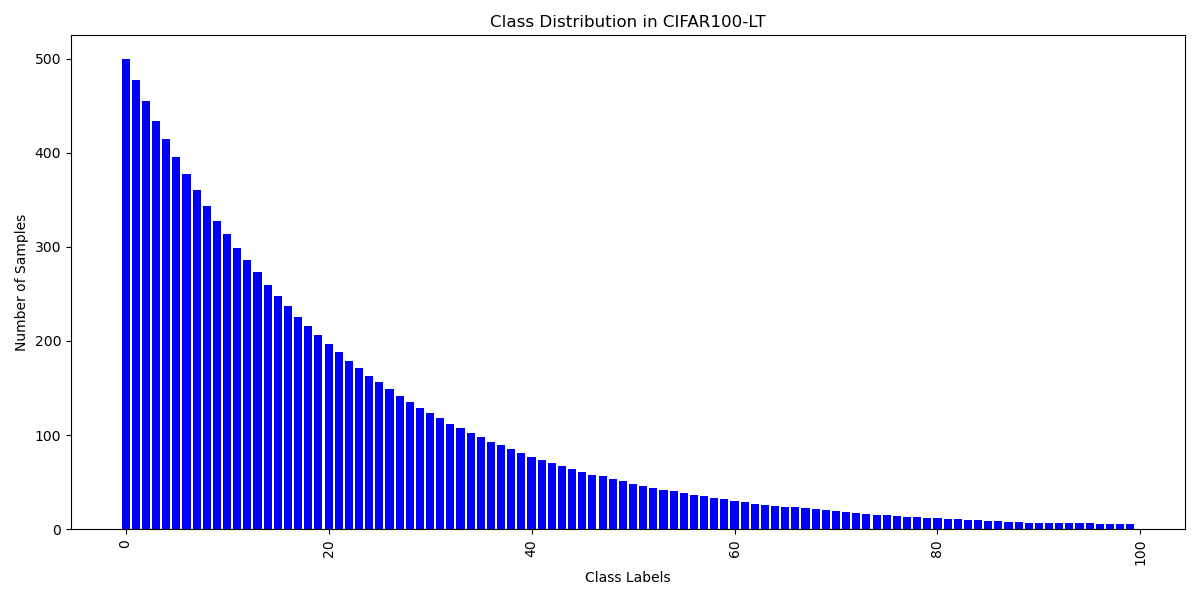
\includegraphics[width=0.9\textwidth]{Images/Plots/Class Distribution for CIFAR100-LT.png}
    \caption{The class distribution of CIFAR100-LT with imbalance ratio 100 generated by the imbalance\_cifar.py in the LDAM-DRW GitHub repository \cite{kaidic_ldam_drw}.}
    \label{fig:cifar100_imbalance_cifar}
\end{figure}

\begin{figure}[H]
    \centering
    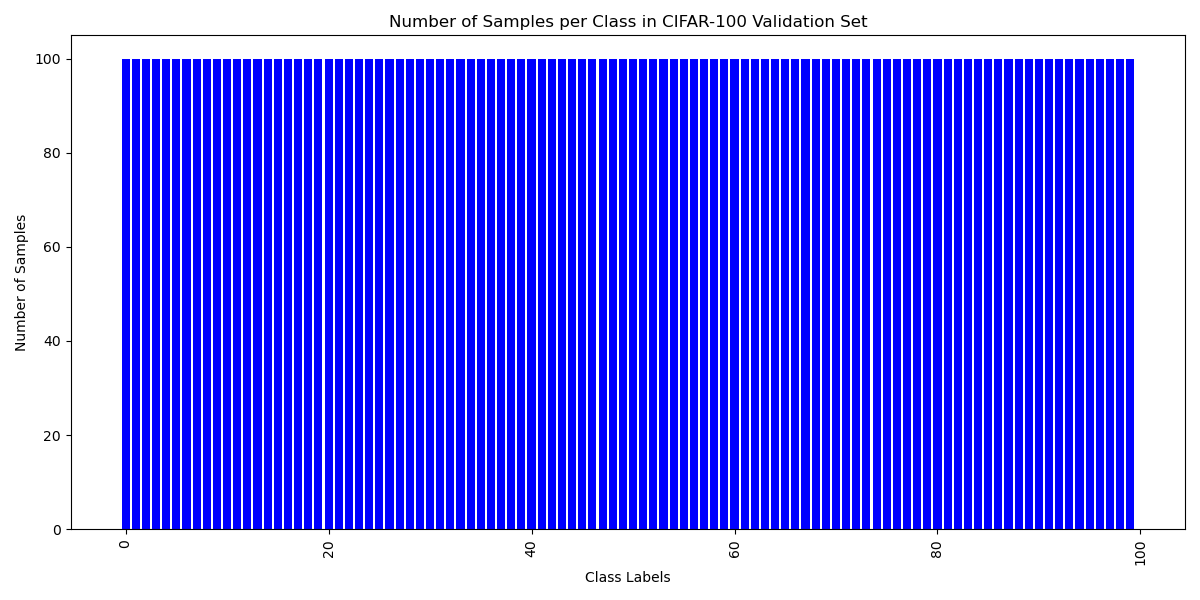
\includegraphics[width=0.9\textwidth]{Images/Plots/cifar100_val_class_distribution.png}
    \caption{The class distribution of the CIFAR100 validation set from torchvision [reference here].}
    \label{fig:cifar100val}
\end{figure}

\subsection{Data Augmentation}
Not sure if this should be a section, or if it should be in the experimental setup section.

Describe what data augmentation was used on the training data.

\section{Long-tailed Learning Techniques}
Description of the specific methods used to address class imbalance, such as data sampling, class re-weighting, etc. 
Justification for selecting these techniques, potentially referencing prior research (from Deep Long-Tailed Learning: A Survey by Zhang et al.).

\subsection{Model Selection}
\textit{A list of subjects to include in this section:}

\begin{itemize}
    \item Mention the model architectures chosen for training, and describe why they are appropriate for deep long-tailed learning with reference to the background section.
    \item Discuss the strengths and limitations of these models in addressing the challenges posed by imbalanced data.
    \item Describe how they were pretrained (ImageNet-1K, ImageNet-21K) and what that means for the training on CIFAR100.
\end{itemize}


\subsection{Selection of Loss Function}
\textit{A list of subjects to include in this section:}

 \begin{itemize}
    \item Describe the different loss functions and why they are appropriate for deep long-tailed learning with reference to the background section.
    \item Rationale for each loss function's inclusion, focusing on its expected benefits for imbalanced classes and how it adresses the bias toward majority classes.
 \end{itemize}

\subsection{Excluded Long-Tailed Learning Methods}
This section will explain why some deep long-tailed learning techniques, like re-sampling, was not the focus of this thesis.

\section{Evaluation Metrics}
\textit{A list of subjects to include in this section:}

\begin{itemize}
    \item Describe common evaluation metrics used for classification tasks.
    \item Explain the choice of top-1 accuracy.
    \item Explain how the performance is assessed across different class groups.
    \item Explain the choice of F1-score.
\end{itemize}

\section{Reproducibility}
\textit{A list of subjects to include in this section:}

\begin{itemize}
    \item Use of random seed initialization.
    \item Documentation of dataset versions and codebase.
    \item Availability of scripts for dataset preparation and model training.
\end{itemize}

\section{Implementation Details}
Technical explanations of any unique or customized methods implemented in code, for example the custom dataset.

\textit{A list of subjects to include in this section:}

\begin{itemize}
    \item Explain how the models where implemented.
    \item Rationale for implementing the loss functions manually instead of copy existing repositories.
    \item Describe the benefits of copying existing repositories.
\end{itemize}

